
  %%%%%%%%%%%%%%%%%%%%%%%%%Subject%%%%%%%%%%%%%%%%%%%%%%%%%%%%%%%%%%

  \section{Subject}

  \subsection{Definition}

  \begin{frame}
          \frametitle{Definition}
  \begin{itemize}[<+->]
  \item \textbf{Context:} To model water sterilization by UV radiation with this device :
          \begin{figure}
                  \raggedleft
                  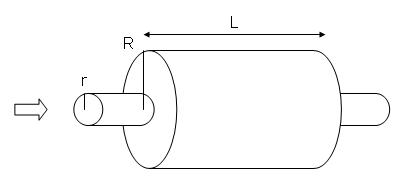
\includegraphics[width=5cm,height=2cm]{./images/sterilisateurh.jpg}
                  \hspace{3mm}
                  \raggedright
                  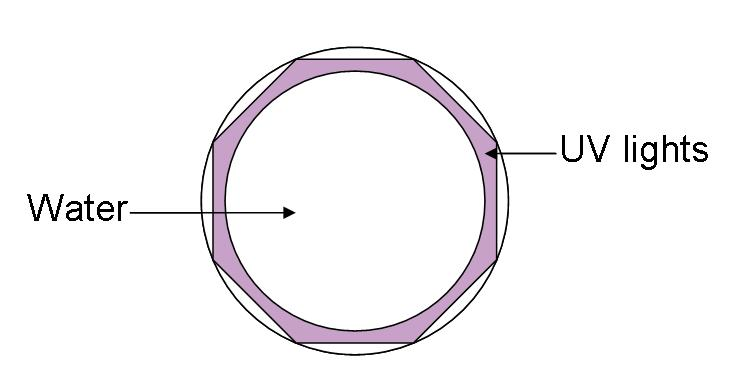
\includegraphics[width=4cm,height=2cm]{./images/coupeSterilisateur.jpg}
          \end{figure}
  \item \textbf{Goal:} To find the optimal radius $r$ and $R$ for which :
          \begin{itemize} 
                  \item[*] At the end of the pipe, the water is sterilized.
                  \item[*] The flow must be 2 or 4 $l.min^{-1}$.
                  \item[*] $R \in [7mm - 20mm]$ and $r \in [2mm - 6mm]$
          \end{itemize}
  \item \textbf{Expected Result:} To create a computer program to search these radius.
  \end{itemize}
  \end{frame}

  \subsection{Methodology}

  \begin{frame}
          \frametitle{Methodology}
  \begin{block}{Different concerned domains:}
  \begin{itemize}[<+->]
  \item Micro-Biology (bacteria's concentration)
  \item Fluid Mechanics
  \item Radiation
  \end{itemize}
  \end{block}
  \pause
  \invisible<1-2> {Our research approach: }
  \begin{block}{Simplified case $\Rightarrow$ real case:}
  \begin{itemize}[<+->]
  \item 0D mean velocity
  \item 1D mean velocity
  \item 2D axisymmetric with a Poiseuille's Profile
  \item 2D axisymmetric with simplified Navier-Stokes' equations
  \end{itemize}
  \end{block}
  \end{frame}


  \begin{frame}
          \frametitle{Methodology}
          \begin{figure}
                  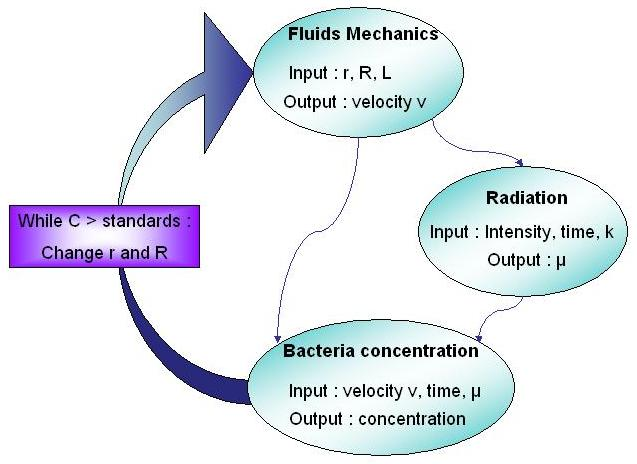
\includegraphics[width=9cm,height=7cm]{./images/methodology2.jpg}
          \end{figure}
  \end{frame}

  \subsection{Objectives}
  \begin{frame}
  \frametitle{Objectives}
  \underline{\textbf{\color{blue}First:}}\\
  \vspace{5mm}
  $\Rightarrow$ To complete the 0D model before mid-February.\\
  \vspace{4mm}
  $\Rightarrow$ To finish the 2D model and give representative results for $r$ and $R$ to obtain sterilised water.\\
  \vspace{8mm}
  \underline{\textbf{\color{blue}If miracle:}}\\
  \vspace{5mm}
  $\Rightarrow$ To do the same with the 3D model.\end{frame}
